\documentclass[11pt,a4paper]{ctexart}
\usepackage[utf8]{inputenc}
\usepackage{geometry}
\geometry{left=2.5cm,right=2.5cm,top=2.8cm,bottom=2.8cm}
\usepackage{amsmath,amssymb,amsfonts}
\usepackage{enumitem}
\usepackage{titlesec}
\usepackage{xcolor}
\usepackage{tcolorbox}
\usepackage{hyperref}

% 引入画图和绝对位置放置宏包用于生成水印
\usepackage{graphicx}
\usepackage{eso-pic}
\usepackage{tikz} % 引入 TikZ 宏包用于绘图

% 解决带圈数字在部分编译器下报错的问题
\xeCJKDeclareCharClass{CJK}{"2460->"2469}

% --- 颜色定义 ---
\definecolor{mainblue}{RGB}{26, 82, 118}
\definecolor{secblue}{RGB}{41, 128, 185}
\definecolor{bglight}{RGB}{244, 246, 247}
\definecolor{textdark}{RGB}{44, 62, 80}

% --- 页面美化与字体设置 ---
\hypersetup{colorlinks=true, linkcolor=mainblue, urlcolor=secblue}
\setlist[itemize]{leftmargin=2em, itemsep=0.3em}
\setlist[enumerate]{leftmargin=2em, itemsep=0.3em}

% --- 标题样式自定义 ---
\titleformat{\section}{\large\bfseries\color{mainblue}}{\thesection}{1em}{}[{\color{mainblue}\titlerule[1pt]}]
\titleformat{\subsection}{\normalsize\bfseries\color{secblue}}{\thesubsection}{1em}{}
\titleformat{\subsubsection}{\small\bfseries\color{textdark}}{\thesubsubsection}{1em}{}

% --- 水印设置 (每页三个，斜45度，居中分布) ---
\newcommand{\WMText}{贺昱琪学习资料}
\newcommand{\WMScale}{2.28}
\newcommand{\WMAngle}{45}
\colorlet{WMColor}{black!8}

\AddToShipoutPictureBG{%
  \AtPageLowerLeft{%
    \put(\LenToUnit{0.66\paperwidth},\LenToUnit{0.70\paperheight}){%
      \rotatebox{\WMAngle}{\scalebox{\WMScale}{\textcolor{WMColor}{\WMText}}}%
    }%
    \put(\LenToUnit{0.33\paperwidth},\LenToUnit{0.50\paperheight}){%
      \rotatebox{\WMAngle}{\scalebox{\WMScale}{\textcolor{WMColor}{\WMText}}}%
    }%
    \put(\LenToUnit{0.66\paperwidth},\LenToUnit{0.30\paperheight}){%
      \rotatebox{\WMAngle}{\scalebox{\WMScale}{\textcolor{WMColor}{\WMText}}}%
    }%
  }%
}

\begin{document}

\begin{center}
    \LARGE \textbf{贺昱琪专项训练一}
\end{center}

\vspace{0.5cm}

\noindent \textbf{一、认真填一填（每小题 3 分，共 30 分）}

\begin{enumerate}
    \item 在 $0.4\dot{3}$、$\frac{43}{100}$、$43.3\%$、$0.434$ 这组数中，最大数与最小数的差是\underline{\hspace{2cm}}。\vspace{1.2cm}
    
    \item 把 $\frac{3}{5}$ 的分母增加 10，要使分数的值不变，则分子应该增加\underline{\hspace{2cm}}。\vspace{1.2cm}
    
    \item 
    \begin{minipage}{0.65\textwidth}
        图1为一正面白色，反面灰色的长方形纸片，今沿虚线剪开分成甲、乙两个长方形纸片，并将甲纸片反面朝上粘贴于乙纸片上，形成一张白、灰相间的长方形纸片，如图2所示。若图2中的白色与灰色区域面积比为 $10 : 3$，图2纸片的面积为 39，则图1纸片的面积为\underline{\hspace{2cm}}。
    \end{minipage}
    \hfill
    \begin{minipage}{0.3\textwidth}
        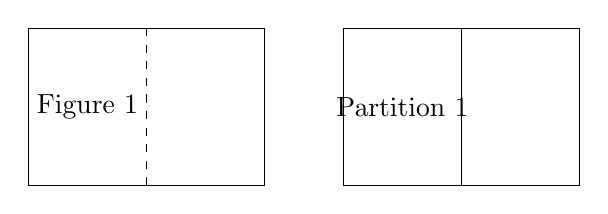
\begin{tikzpicture}
          \draw (0,0) rectangle (3,2);
          \draw[dashed] (1.5,0) -- (1.5,2);
          \node at (0.75, 1) {Figure 1};
          \begin{scope}[xshift=4cm]
            \draw (0,0) rectangle (3,2);
            \draw (1.5,0) -- (1.5,2);
            \node at (0.75, 1) {Partition 1};
          \end{scope}
        \end{tikzpicture}
    \end{minipage}
    
    \item 
    \begin{minipage}{0.65\textwidth}
        如图，点 $P$ 为长方形 $ABCD$ 上的一个动点，它以每秒 1cm 的速度从点 $A$ 出发，沿着 $A \rightarrow B \rightarrow C \rightarrow D$ 的路线运动，到 $D$ 点停止。从 2 秒开始一直至 6 秒 $\triangle PAD$ 的面积均为 4 平方厘米。长方形 $ABCD$ 的周长为\underline{\hspace{2cm}}cm。
    \end{minipage}
    \hfill
    \begin{minipage}{0.3\textwidth}
        \begin{tikzpicture}
          \draw (0,0) rectangle (4,3);
          \node at (0,3.2) {A}; \node at (4,3.2) {B}; \node at (4,-0.2) {C}; \node at (0,-0.2) {D};
          \draw[dashed, ->] (0,3) -- (4,3) -- (4,0) -- (0,0);
          \draw[fill=black] (0,3) circle (0.05); \node at (-0.2, 3) {P};
          \draw (0,0) -- (0,3) -- (0,0);
        \end{tikzpicture}
    \end{minipage}
    
    \item 
    \begin{minipage}{0.65\textwidth}
        如图①，$\triangle ABC$ 的三个顶点和它内部点 $P_1$，把 $\triangle ABC$ 分成 3 个互不重叠的小三角形；如图②，$\triangle ABC$ 的三个顶点和它内部点 $P_1$、$P_2$，把 $\triangle ABC$ 分成 5 个互不重叠的小三角形；如图③，$\triangle ABC$ 的三个顶点和它内部点 $P_1$、$P_2$、$P_3$，把 $\triangle ABC$ 分成 7 个互不重叠的小三角形；$\cdots$；$\triangle ABC$ 的三个顶点和它内部点 $P_1$、$P_2$、$P_3$，$\cdots$，$P_{2017}$，把 $\triangle ABC$ 分成\underline{\hspace{2cm}}个互不重叠的小三角形。
    \end{minipage}
    \hfill
    \begin{minipage}{0.3\textwidth}
        \begin{tikzpicture}
          \draw (0,0) -- (4,0) -- (1,3) -- cycle; 
          \node at (-0.2,0) {B}; \node at (4.2,0) {C}; \node at (1,3.2) {A};
          \draw (1,3) -- (1.5,0); 
        \end{tikzpicture}
    \end{minipage}
    
    \item 如图，一个酒瓶里面深 30cm，底面内直径 10cm，瓶里酒深 15cm。把酒瓶塞紧后，使其瓶口向下倒立，这时酒深 25cm，则酒瓶容积是\underline{\hspace{2cm}}立方厘米。\vspace{1.2cm}
    
    \item 如图，是由若干个正方体形状的木块堆成的，平放在桌面上。其中，上面正方体的下底面四个顶点恰是下面相邻正方体上底面各边的中点，如果最下面的正方体棱长为 1，且这些正方体露在外面的面积和超过 8，那么正方体的个数至少是\underline{\hspace{2cm}}个。\vspace{1.2cm}
    
    \item 某班全体学生进行了一次篮球投篮练习，每人投球 10 个。每投进一个球得 1 分。得分的分布情况如下表所示：
    \begin{table}[htbp]
        \centering
        \begin{tabular}{|c|c|c|c|c|c|c|c|}
            \hline
            得分 & 0 & 1 & 2 & $\cdots$ & 8 & 9 & 10 \\
            \hline
            人数 & 7 & 5 & 4 & $\cdots$ & 3 & 4 & 1 \\
            \hline
        \end{tabular}
    \end{table}
    已知该班学生中，至少得 3 分的人平均得 6 分。得分不到 8 分的人平均得分为 3 分。那么该班有\underline{\hspace{2cm}}人。\vspace{1.2cm}
    
    \item 
    \begin{minipage}{0.65\textwidth}
        如图，直角 $\triangle ABC$ 的斜边 $AB$长为 10cm，$\angle ABC=60^\circ$。此时 $BC$ 长 5cm。以 $B$ 点为中心，将 $\triangle ABC$ 顺时针旋转 $120^\circ$，点 $A$、$C$ 分别到达点 $E$、$D$ 的位置，则图中阴影部分的面积为\underline{\hspace{2cm}}。（结果保留 $\pi$）
    \end{minipage}
    \hfill
    \begin{minipage}{0.3\textwidth}
        \begin{tikzpicture}
          \draw (0,0) -- (2,0) -- (2,3.46) -- cycle; 
          \node at (0,-0.2) {B}; \node at (2,-0.2) {C}; \node at (2.2, 3.6) {A};
          \draw (0.5,0.2) arc (0:60:0.5); \node at (0.6, 0.4) {60$^\circ$};
          \begin{scope}[rotate around={-120:(0,0)}]
             \draw (0,0) -- (2,0) -- (2,3.46) -- cycle; 
             \node at (2.2, 3.6) {E}; \node at (2,-0.2) {D};
          \end{scope}
        \end{tikzpicture}
    \end{minipage}
    
    \item 如图算式中，每个汉字代表 1 个数字，不同的汉字代表不同的数字，已知“神”=3，那么被乘数是\underline{\hspace{2cm}}。\\
    \begin{center}
    \begin{tabular}{r@{\quad}l}
      & 神舟五号飞天 \\
      $\times$ & \hspace{2.2cm} 神 \\
      \hline
      & 飞天神舟五号
    \end{tabular}
    \end{center}
\end{enumerate}

\vspace{0.8cm}

\noindent \textbf{二、细心算一算}

\begin{enumerate}
    \item[11.] 计算（每小题 4 分，共 16 分）
    \begin{enumerate}
        \item[(1)] $12 \div \left(-\frac{3}{4}\right) + 2 \div \frac{2}{5} \times \frac{1}{2}$
        \vspace{3.5cm}
        
        \item[(2)] $9 \times \left[ 1 - \left(-\frac{2}{5} + \frac{9}{20}\right) \right] \div \frac{3}{10} - \frac{1}{7}$
        \vspace{3.5cm}
        
        \item[(3)] $\left(\frac{5}{8} \times 60 - 60 \div \frac{8}{21}\right) \times \left(-\frac{1}{2} + \frac{1}{5} - \frac{5}{12}\right)$
        \vspace{3.5cm}
        
        \item[(4)] $2\frac{5}{6} - 3\frac{1}{12} + 4\frac{19}{20} - 5\frac{1}{30} + 6\frac{41}{42} - \frac{1}{2}$
        \vspace{3.5cm}
    \end{enumerate}
\end{enumerate}

\vspace{0.8cm}

\noindent \textbf{三、用心想一想}

\begin{enumerate}
    \item[12.] (7分) 为增强居民节约用水意识，某市在 2017 年开始对供水范围内的居民用水实行“阶梯收费”。具体收费标准如下表：
    \begin{table}[htbp]
        \centering
        \begin{tabular}{|l|l|}
            \hline
            一户居民一个月用水量记为 $x$ 立方米 & 水费单价（单位：元/立方米） \\
            \hline
            $x \le 22$ & $a$ \\
            \hline
            超出 22 立方米的部分 & $a+1.1$ \\
            \hline
        \end{tabular}
    \end{table}
    某户居民四月份用水 10 立方米时，缴纳水费 23 元。
    \begin{enumerate}
        \item[(1)] 求 $a$ 值；
        \vspace{3.0cm}
        
        \item[(2)] 若该用户五月份所缴水费为 71 元，求该户居民五月份的用水量。
        \vspace{3.5cm}
    \end{enumerate}
    
    \item[13.] (8分) 星期天，小强骑自行车到郊外与同学一起游玩。从家出发 2 小时到达目的地，游玩 3 小时后按原路以原速返回。小强离家 4 小时 40 分钟后，妈妈驾车沿相同的路线迎小强。已知小强骑车的速度为 15 千米/小时，妈妈驾车的速度为 60 千米/小时。
    \begin{enumerate}
        \item[(1)] 小强家与游玩地距离是多少？
        \vspace{3.0cm}
        
        \item[(2)] 妈妈出发多长时间与小强相遇？
        \vspace{3.5cm}
    \end{enumerate}

    \item[14.] (8分) 单独完成一项任务，甲按规定时间可提前 2 天完成，乙则要超过规定时间 3 天才能完成。如果甲、乙二人合作 2 天后，剩下的由乙单独做，那么刚好在规定时间完成。问：甲、乙二人合作需多少天完成？
    \vspace{4.5cm}
\end{enumerate}

\vspace{0.8cm}

\noindent \textbf{四、勇敢闯一闯}

\begin{enumerate}
    \item[15.] (9分) 问题提出：如何把一个正方形分割成 $n (n \ge 6)$ 个小正方形？
    
    为解决上面问题，我们先来研究两种简单的“基本分割线”。
    
    基本分割法1：如图1，把一个正方形分割成 4 个小正方形，即在原来 1 个正方形的基础上增加 3 个正方形；
    
    基本分割法2：如图2，把一个正方形分割成 6 个小正方形，即在原来 1 个正方形的基础上增加 5 个正方形。
    
    解决问题：有了上述两种“基本分割法”后，我们就可以把一个正方形分割成 $n (n \ge 6)$ 个小正方形。
    \begin{enumerate}
        \item[(1)] 把一个正方形分割成 9 个小正方形。
        \vspace{4.0cm}
        
        \item[(2)] 把一个正方形分割成 10 个小正方形。
        \vspace{4.0cm}
        
        \item[(3)] 把一个正方形分割成 11 个小正方形。
        \vspace{4.0cm}
    \end{enumerate}
    (注：用签字笔和直尺画出示意图即可，不用说明分割方法)
    
    \item[16.] (10分) 某房地产开发商开发一套房子的成本随着物价上涨比原来增加了 10\%，为了赚钱，开发商把售价提高了 0.5 倍，利润率比原来增加了 60\%，求开发商原来的利润率。
    \vspace{4.5cm}

    \item[17.] (12分) 问题情境
    
    如图1，$\triangle ABC$ 中，沿 $\angle BAC$ 的平分线 $AB_1$ 折叠，剪掉重叠部分；将余下部分沿 $\angle B_1A_1C$ 的平分线 $A_1B_2$ 折叠，剪掉重叠部分；如此反复操作，沿 $\angle B_nA_nC$ 的平分线 $A_nB_{n+1}$ 折叠，点 $B_n$ 与点 $C$ 重合，我们就称 $\angle BAC$ 是 $\triangle ABC$ 的正角。
    
    以图2为例，$\triangle ABC$ 中，$\angle B=70^\circ$，$\angle C=35^\circ$。若沿 $\angle BAC$ 的平分线 $AB_1$ 折叠，则 $\angle AA_1B_1=70^\circ$。沿 $A_1B_1$ 剪掉重叠部分，在余下的 $\triangle B_1A_1C$ 中，由三角形的内角和定理可知 $\angle A_1B_1C=35^\circ$，若沿 $\angle B_1A_1C$ 的平分线 $A_1B_2$ 第二次折叠，则点 $B_1$ 与 $C$ 重合。此时，我们就称 $\angle BAC$ 是 $\triangle ABC$ 的正角。
    
    \vspace{0.3cm}
    \noindent 探究发现
    \begin{enumerate}
        \item[(1)] $\triangle ABC$ 中，$\angle B=2\angle C$，则经过两次折叠后，$\angle BAC$ 是不是 $\triangle ABC$ 的正角？\underline{\hspace{2cm}}（填“是”或“不是”）；
        \vspace{2.5cm}
        
        \item[(2)] 小明经过三次折叠发现 $\angle BAC$ 是 $\triangle ABC$ 的正角，则 $\angle B$ 与 $\angle C$ (不妨设 $\angle B > \angle C$) 之间的等量关系为\underline{\hspace{3cm}}；\\
        根据以上内容猜想：若经过 $n$次折叠 $\angle BAC$ 是 $\triangle ABC$ 的正角，则 $\angle B$ 与 $\angle C$ (不妨设 $\angle B > \angle C$) 之间的等量关系为\underline{\hspace{3cm}}。
        \vspace{3.5cm}
    \end{enumerate}
    
    \noindent 应用提升
    \begin{enumerate}
        \item[(3)] 如果一个三角形的最小角是 $15^\circ$，直接写出此三角形另外两个角的度数，使得此三角形的三个角均是它的正角。
        \vspace{3.5cm}
    \end{enumerate}
\end{enumerate}

\end{document}